\chapter{Introduction}

\section{What are Boids?}

\begin{minipage}{0.99\textwidth}
    \begin{itemize}
        \item Introduced by Craig Reynolds in 1986
        \item Simulates flocking behavior of birds, fish, or other organisms
    \end{itemize}
    \begin{center}
        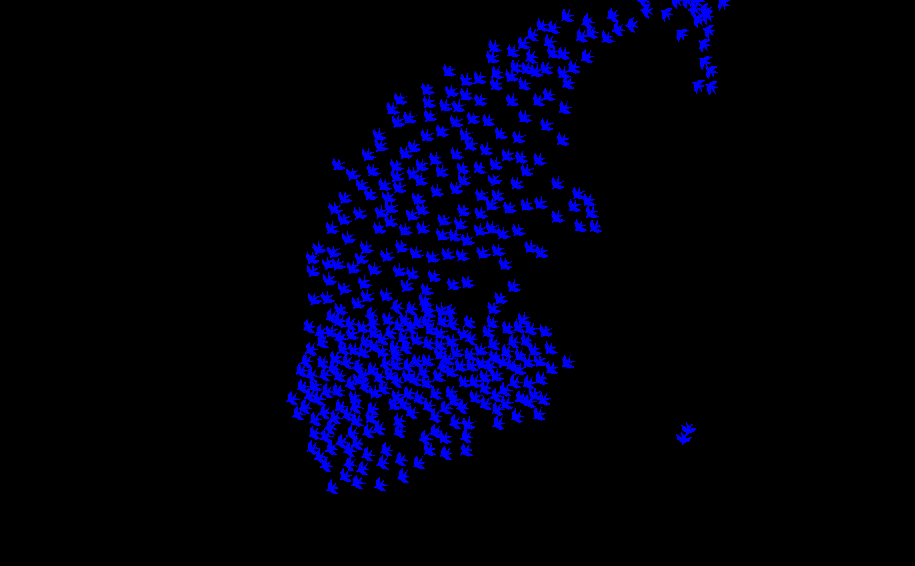
\includegraphics[width=0.7\textwidth]{../../images/boidsvisualizzationexample.png}
    \end{center}
\end{minipage}

\section{The Three Fundamental Rules}

\begin{itemize}
    \item \textbf{Alignment}: Each boid tries to match its velocity (direction and speed) to the average velocity of its local neighbors. This causes the group to move in a similar direction, promoting coordinated movement.
    \item \textbf{Cohesion}: Each boid steers towards the average position (center of mass) of its nearby flockmates. This keeps the group together and prevents individuals from straying too far from the flock.
    \item \textbf{Separation}: Each boid actively avoids crowding by steering away from neighbors that are too close. This prevents collisions and maintains a comfortable distance between individuals.
\end{itemize}

\vspace{0.5cm}
Each boid follows these rules independently, creating realistic flocking patterns without central control.

\section{Project Goals}

\begin{itemize}
    \item Implement efficient Boids simulation in C++
    \item Compare sequential vs parallel implementations
    \item Analyze different data layouts: Array of Structures (AoS) vs Structure of Arrays (SoA)
    \item Evaluate performance scalability with OpenMP
    \item Utilize SIMD optimizations where possible
\end{itemize}

\section{Implementation Overview}

\textbf{Technologies Used:}
\begin{itemize}
    \item \textbf{Language}: C++ for performance
    \item \textbf{Parallelization}: OpenMP for multi-core optimization
    \item \textbf{Visualization}: SFML (Simple and Fast Multimedia Library)
    \item \textbf{Build System}: CMake for cross-platform compilation
\end{itemize}

